\documentclass[conference]{IEEEtran}
\IEEEoverridecommandlockouts
% The preceding line is only needed to identify funding in the first footnote. If that is unneeded, please comment it out.
\usepackage{cite}
\usepackage{amsmath,amssymb,amsfonts}
\usepackage{algorithmic}
\usepackage{graphicx}
\usepackage{textcomp}
\usepackage{xcolor}
\def\BibTeX{{\rm B\kern-.05em{\sc i\kern-.025em b}\kern-.08em
    T\kern-.1667em\lower.7ex\hbox{E}\kern-.125emX}}
\begin{document}

\title{Comparison of three selected ML models for predicting decision of the Dean}

\author{\IEEEauthorblockN{inż. Jan Łukomski}
\IEEEauthorblockA{\textit{Faculty of Electrical Engineering} \\
\textit{Warsaw Univerity of Technology}\\
Warsaw, Poland}
\and
\IEEEauthorblockN{inż. Paweł Podgórski}
\IEEEauthorblockA{\textit{Faculty of Electrical Engineering} \\
\textit{Warsaw Univerity of Technology}\\
Warsaw, Poland}
}

\maketitle

\begin{abstract}
%% TODO: abstract
\end{abstract}

\begin{IEEEkeywords}
ml, svm, knn, decision tree classifier
\end{IEEEkeywords}

\section{Introduction}
Predicting the decision of the Dean in an academic institution is a task of significant importance, as it can greatly influence the lives of students, faculty, and the overall direction of the institution. This article presents a comparative analysis of three carefully selected ML models - Support Vector Machines (SVM), Decision Tree Classifier, and k-nearest neighbors (KNN) - to determine their effectiveness in predicting the Dean's decision as either positive or negative. By examining the performance, strengths, and limitations of each model, this study aims to provide valuable insights that can enhance decision-making processes within academic institutions.

\section{Data cleaning}

\subsection{Decision}
Our first step was to recognize if the decision of Dean was positive or negative.
From all of text representation of decision, we  choose  as positive decisions: 'Zamkniêty - decyzja pozytywna', 'Zamkniêty - inne', 'Decyzja pozytywna - oczekuje na realizacjê' and as negative desicions: 'Zamkniêty - decyzja negatywna', 'Zamkniêty - odrzucony formalnie', 'Zwrócony do korekty'.
We made a new column of type boolean where we indicate if decision was positive or negative.

\subsection{Data transformation}
There is 42 columns in dataset. Most of columns data types are \textit{string} like in "Mode of study", "Language", "Type of application", and some of them are of type \textit{float64}, e.g. "Attachments", "How many changes of statuses", "Missing ECTS".
Using \textit{pd.factorize()} method unique values from each columns were extracted, and their codes. Replacing existing values from column, with the code value. In that way text data was converted into categorical data. That method was used to transform data of columns: 'Mode of study ', 'Level of study (I - Engineering, M - Master)', 'Language' , 'Specialization', 'Type of application', 'Word regulation in substantation', 'Word formal in substantation', 'Word progress in substantation', 'Was the appeal submitted', 'Registration semester', 'Semester of study', 'Word family in substantation', 'Word health in substantation', 'Word family in substantation.1', 'Word accident in substantation', 'Word work in substantation', 'Word promise  in substantation'.

\section{Selecting features}
% features selection description for the prediction problem (this is EDA) - here you should select most interesting features relevant for the specific type of application type using for the simplest case correlation coefficients
% EDA of selected features - here you should try to analyze the dependence of the features on the target value (the deans decision)

\begin{figure}
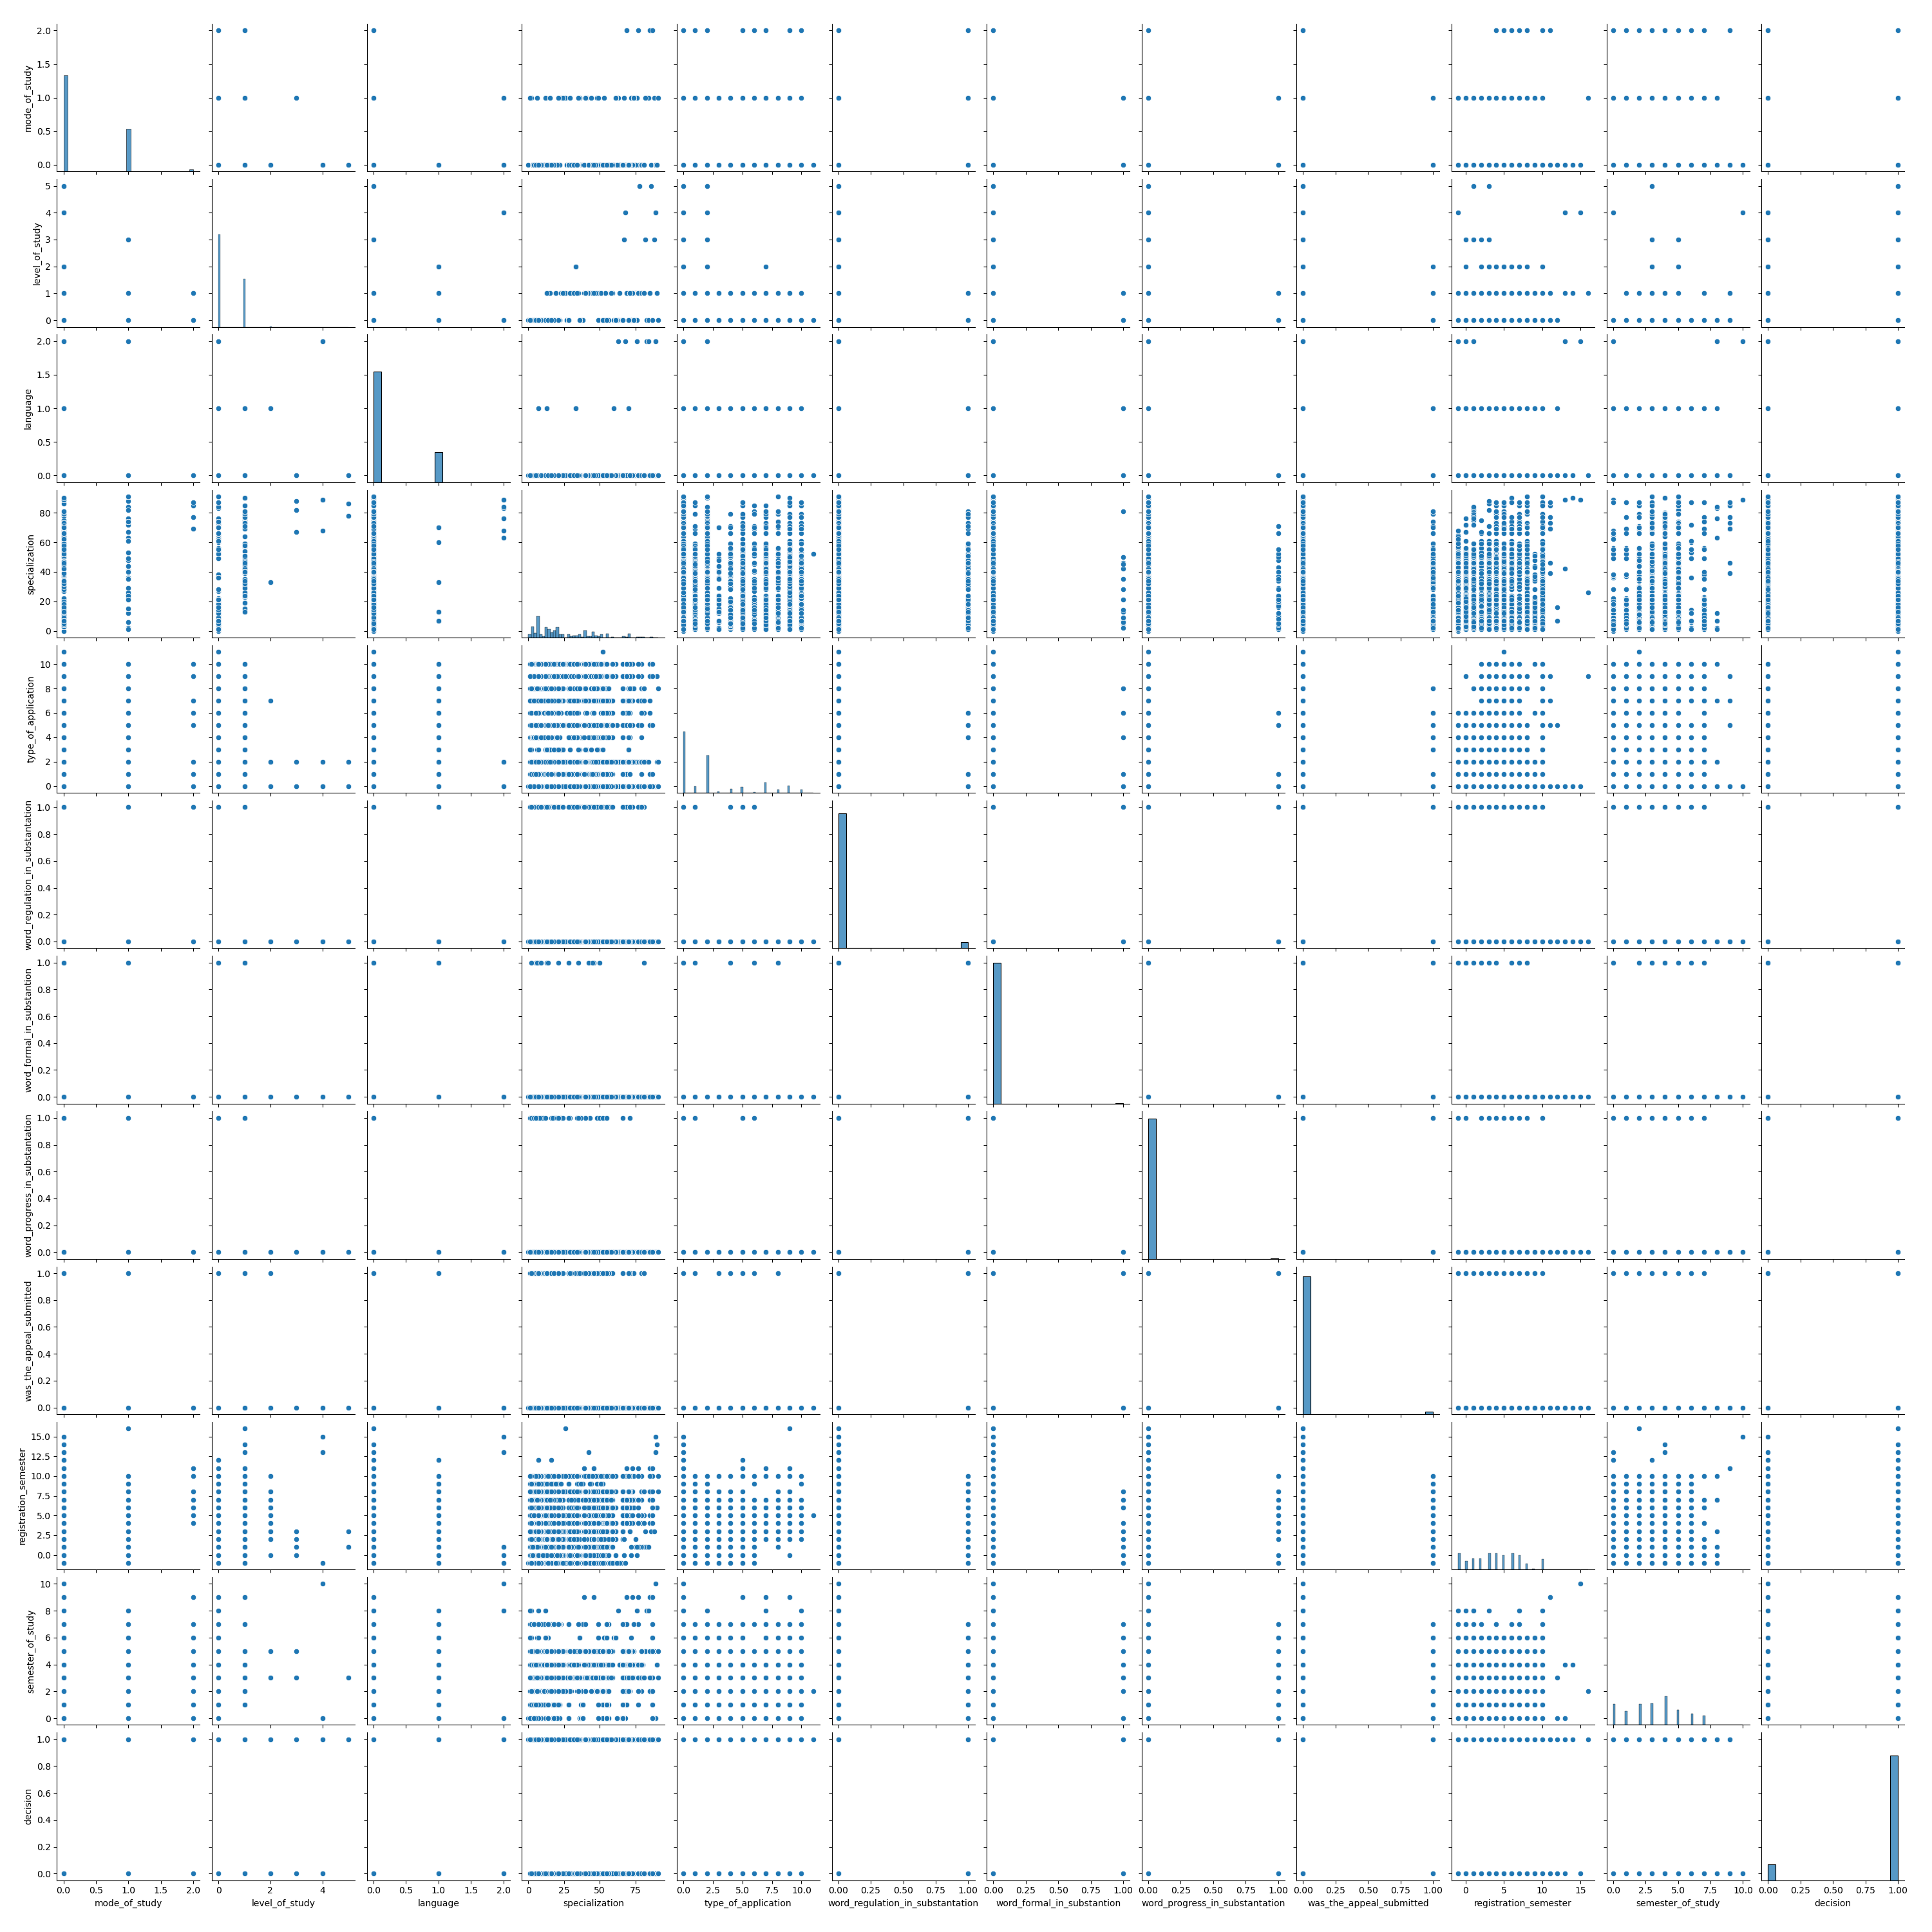
\includegraphics[width=0.5\textwidth]{img/pairplot.png}
\caption{Pairplot of all columns in dataset}
\label{fig}
\end{figure}

\section{Choosen algorithms and testing}
% selection and short theoretical description of two algorithms for the evaluation
% description of the benchmarking experiment - what are you going to check, verify and how you are going to get reasonable the results (eg. performance (classification metrics)),
According to sklearn library recomandation \cite{sklearn} and \cite{towards_class}, we choose to test dataset with SVM model, Decision Tree Classifier and with KNN Classificator.
% generated - to be fixed
The experiment will proceed in several steps. Firstly, the dataset will be preprocessed, involving tasks such as data cleaning, handling missing values, and feature engineering. This step is crucial in ensuring the quality and integrity of the data used for training and testing the ML models.
Next, the dataset will be divided into training and testing sets using an appropriate splitting technique, such as stratified sampling, to maintain the distribution of positive and negative decisions in both sets. The training set will be used to train the ML models, while the testing set will be kept separate and used later for evaluating the models' performance.
Each ML model (SVM, Decision Tree Classifier, and KNN Classifier) will then be trained on the training set using suitable hyperparameter tuning techniques to optimize their performance. Cross-validation may also be employed to estimate the models' generalization capabilities.
Once the models are trained, they will be evaluated using various performance metrics, including accuracy, precision, recall, and F1 score. These metrics provide a comprehensive understanding of the models' predictive capabilities and their ability to correctly classify positive and negative decisions made by the Dean.v

\section{Evaluation}
% tables with prediction results - showing that you have correctly applied the methods,
% tables evaluating performance (prediction metrics) for different types of application forms and both algorithms – this is the main part of the benchmark section,

\begin{figure}
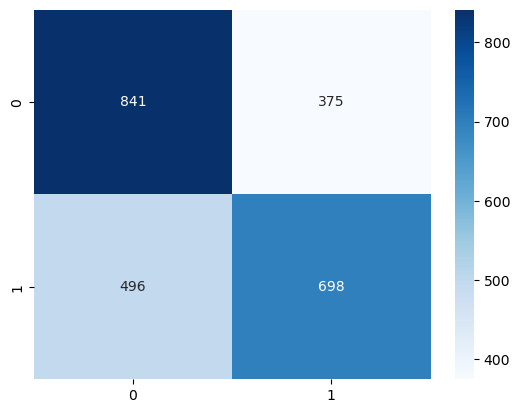
\includegraphics[width=0.5\textwidth]{img/svm_pred.png}
\caption{SVM model prediction}
\label{fig}
\end{figure}

\begin{figure}
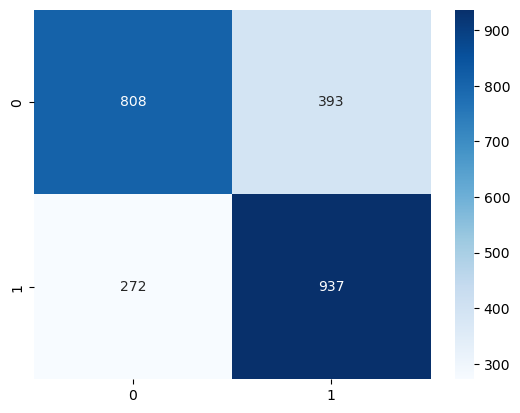
\includegraphics[width=0.5\textwidth]{img/dec_pred.png}
\caption{Decision Tree Classifier prediction}
\label{fig}
\end{figure}

\begin{figure}
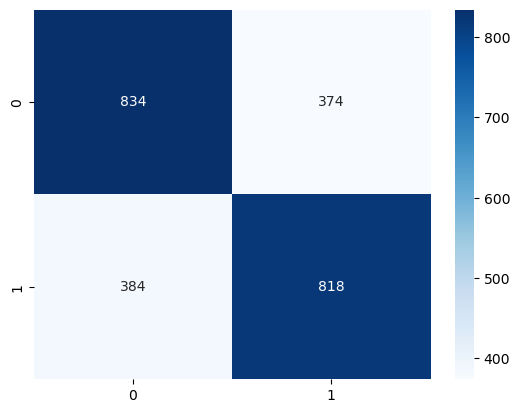
\includegraphics[width=0.5\textwidth]{img/knn_pred.png}
\caption{KNN Classifier prediction}
\label{fig}
\end{figure}

\begin{table}[htbp]
    \centering
    \caption{Comparison of ML Models}
    \label{tab:ml_comparison}
    \begin{tabular}{lccc}
        \hline
        \textbf{Model} & \textbf{Accuracy} & \textbf{Precision} & \textbf{Recall} \\
        \hline
        SVM & 0.64 & 0.64 & 0.64 \\
        Decision Tree Classifier & 0.72 & 0.73 & 0.73 \\
        KNN Classifier & 0.69 & 0.69 & 0.69 \\
        \hline
    \end{tabular}
\end{table}

\begin{table}[htbp]
    \centering
    \caption{Comparison of ML Models}
    \label{tab:ml_comparison}
    \begin{tabular}{lccc}
        \hline
        \textbf{Model} & \textbf{Accuracy} & \textbf{Precision} & \textbf{Recall} \\
        \hline
        SVM & 0.64 & 0.64 & 0.64 \\
        Decision Tree Classifier & 0.72 & 0.73 & 0.73 \\
        KNN Classifier & 0.69 & 0.69 & 0.69 \\
        \hline
    \end{tabular}
\end{table}


\section{Summary}
% summary section (four to five sentences summing up the main outcomes of the paper - stress out the most important features, features which appeared to important by intuition but finally results in poor correlation, best performing algorithm,etc…)
The comparative analysis of three ML models for predicting the dean's decision revealed varying levels of performance. The Decision Tree Classifier outperformed the other models, achieving an accuracy of 0.72, precision of 0.73, and recall of 0.73. The SVM model demonstrated moderate performance with an accuracy, precision, and recall of 0.64. The KNN Classifier achieved similar results to the SVM model, with an accuracy, precision, and recall of 0.69. These findings suggest that the Decision Tree Classifier may be the most effective choice for predicting the dean's decision, considering its higher accuracy and precision values.

\begin{thebibliography}{00}
% literature section should contain at least 4 to 5 positions from Google Scholar!
\bibitem{sklearn} https://scikit-learn.org/stable/tutorial/machine\_learning\_map/index.html
\bibitem{towards_class} https://towardsdatascience.com/top-10-binary-classification-algorithms-a-beginners-guide-feeacbd7a3e2

\end{thebibliography}

\end{document}